\documentclass{./source/Report}

\name{许子绎、王励劼、陈科}
\date{\today}
\course{面向对象程序设计}
\instructor{陈奇}
\expname{文本编辑器}%实验名称

\begin{document}

\makecover

\tableofcontents

\newpage

\section{需求分析}

\subsection{要求}
实现文本编辑器
\subsection{功能}
\begin{enumerate}
    \item 支持基本的文本编辑功能,包括输入、回退、插入、删除、撤销、重做等
    \item 支持文件的保存和打开
    \item 支持搜索与替换
    \item 支持文字格式的设置,包括大小、字体、颜色等
    \item 支持排版设置,包括对齐方式、自动分页等
\end{enumerate}

\section{总体设计}
\subsection{代码结构设计}
使用Qt6.5.0配合Qt Creator生成标准结构的项目代码。使用CMakeLists编译,build文件夹内为本地构建项目目录,src文件夹内放置源文件和头文件、贴图和格式文件。其中images.qrc文件能够读取image文件夹内的贴图(jpg,png,etc.),styles.qrc能够读取styles文件夹内css格式文件。
\begin{figure}[!htbp]
    \begin{minipage}{0.45\textwidth}
        \centering
        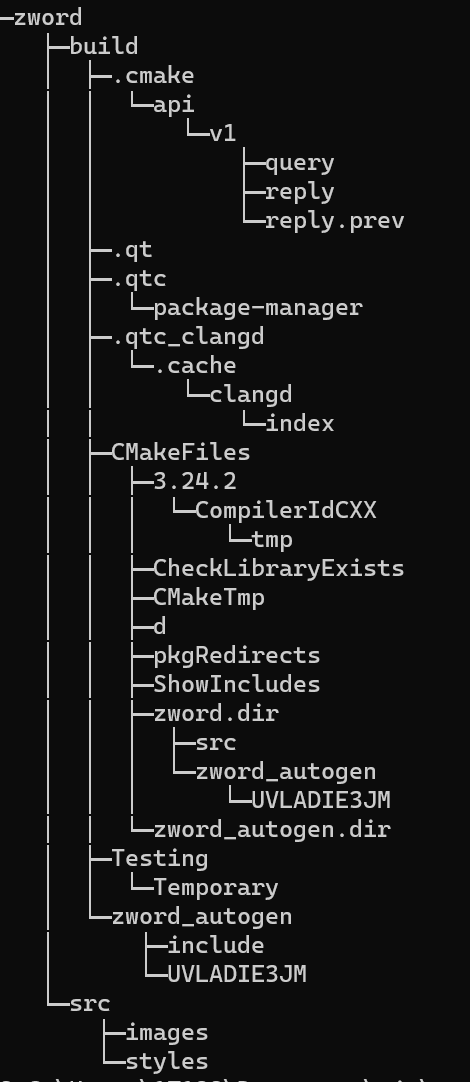
\includegraphics[width=1.5in, height=3in]{1686926262704}
        \caption{项目文件目录}
    \end{minipage}
    \begin{minipage}{0.45\textwidth}
        \centering
        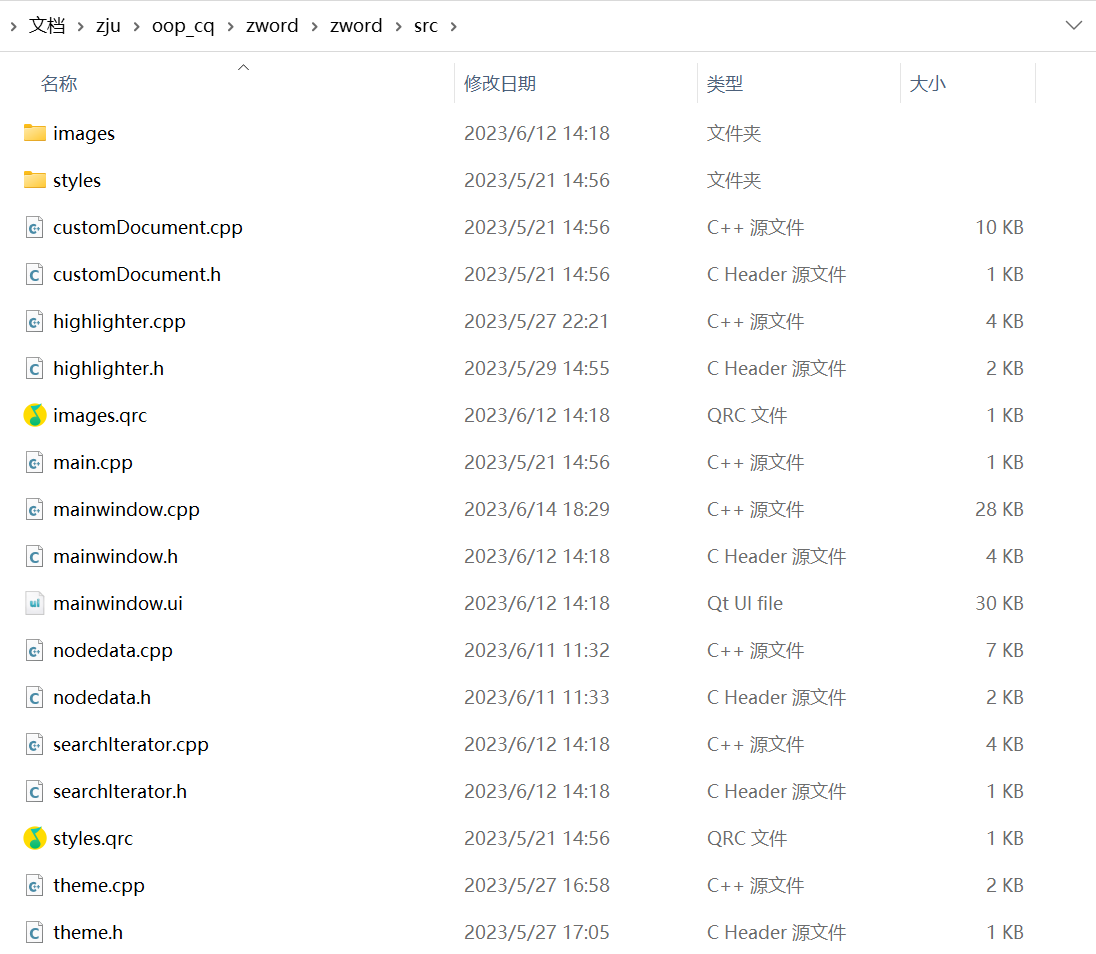
\includegraphics[width=2.5in]{1686926280473}
        \caption{src目录下文件}
    \end{minipage}
\end{figure}
\subsection{实现关键点}
\subsubsection{设计的面向对象}
我们在设计该文本编辑器的最初就希望构建一个能够一次性打开多个在不同文件夹中的笔记文本并进行编辑的。该文本编辑器意图面向希望能够快速进行便签记录,并对不同便签信息进行简单格式编辑和更改,做快速存储功能。
\subsubsection{界面ui设计}
我们使用了Qt自带的ui格式进行设置,只需要进行基本模块的拖动以及模块之间位置和格式关系的设置即可显示页面。在mainwindow.ui中可以进行操作,操作能够自动通过正则表达式存储。\par
Qt中我们主要用到的模块有按键(Buttons)、标签(Label)、ListView和TextEdit。其中TextEdit能够通过Qt自带的提升操作,自动在ui文件中设置自定义的派生类(我们派生为CustomDocument)。而主要运用到的格式关系有Spacers和Layouts,能够分别提供模块的格式拉升功能和多个模块的排版。下图为mainwindow.ui的主要界面设计,可以注意到中间为我们设计的界面,右侧则为我们所加入的各种模块及其之间的关系。
\begin{figure}[!htbp]
    \centering
    \begin{minipage}{0.45\textwidth}
        \centering
        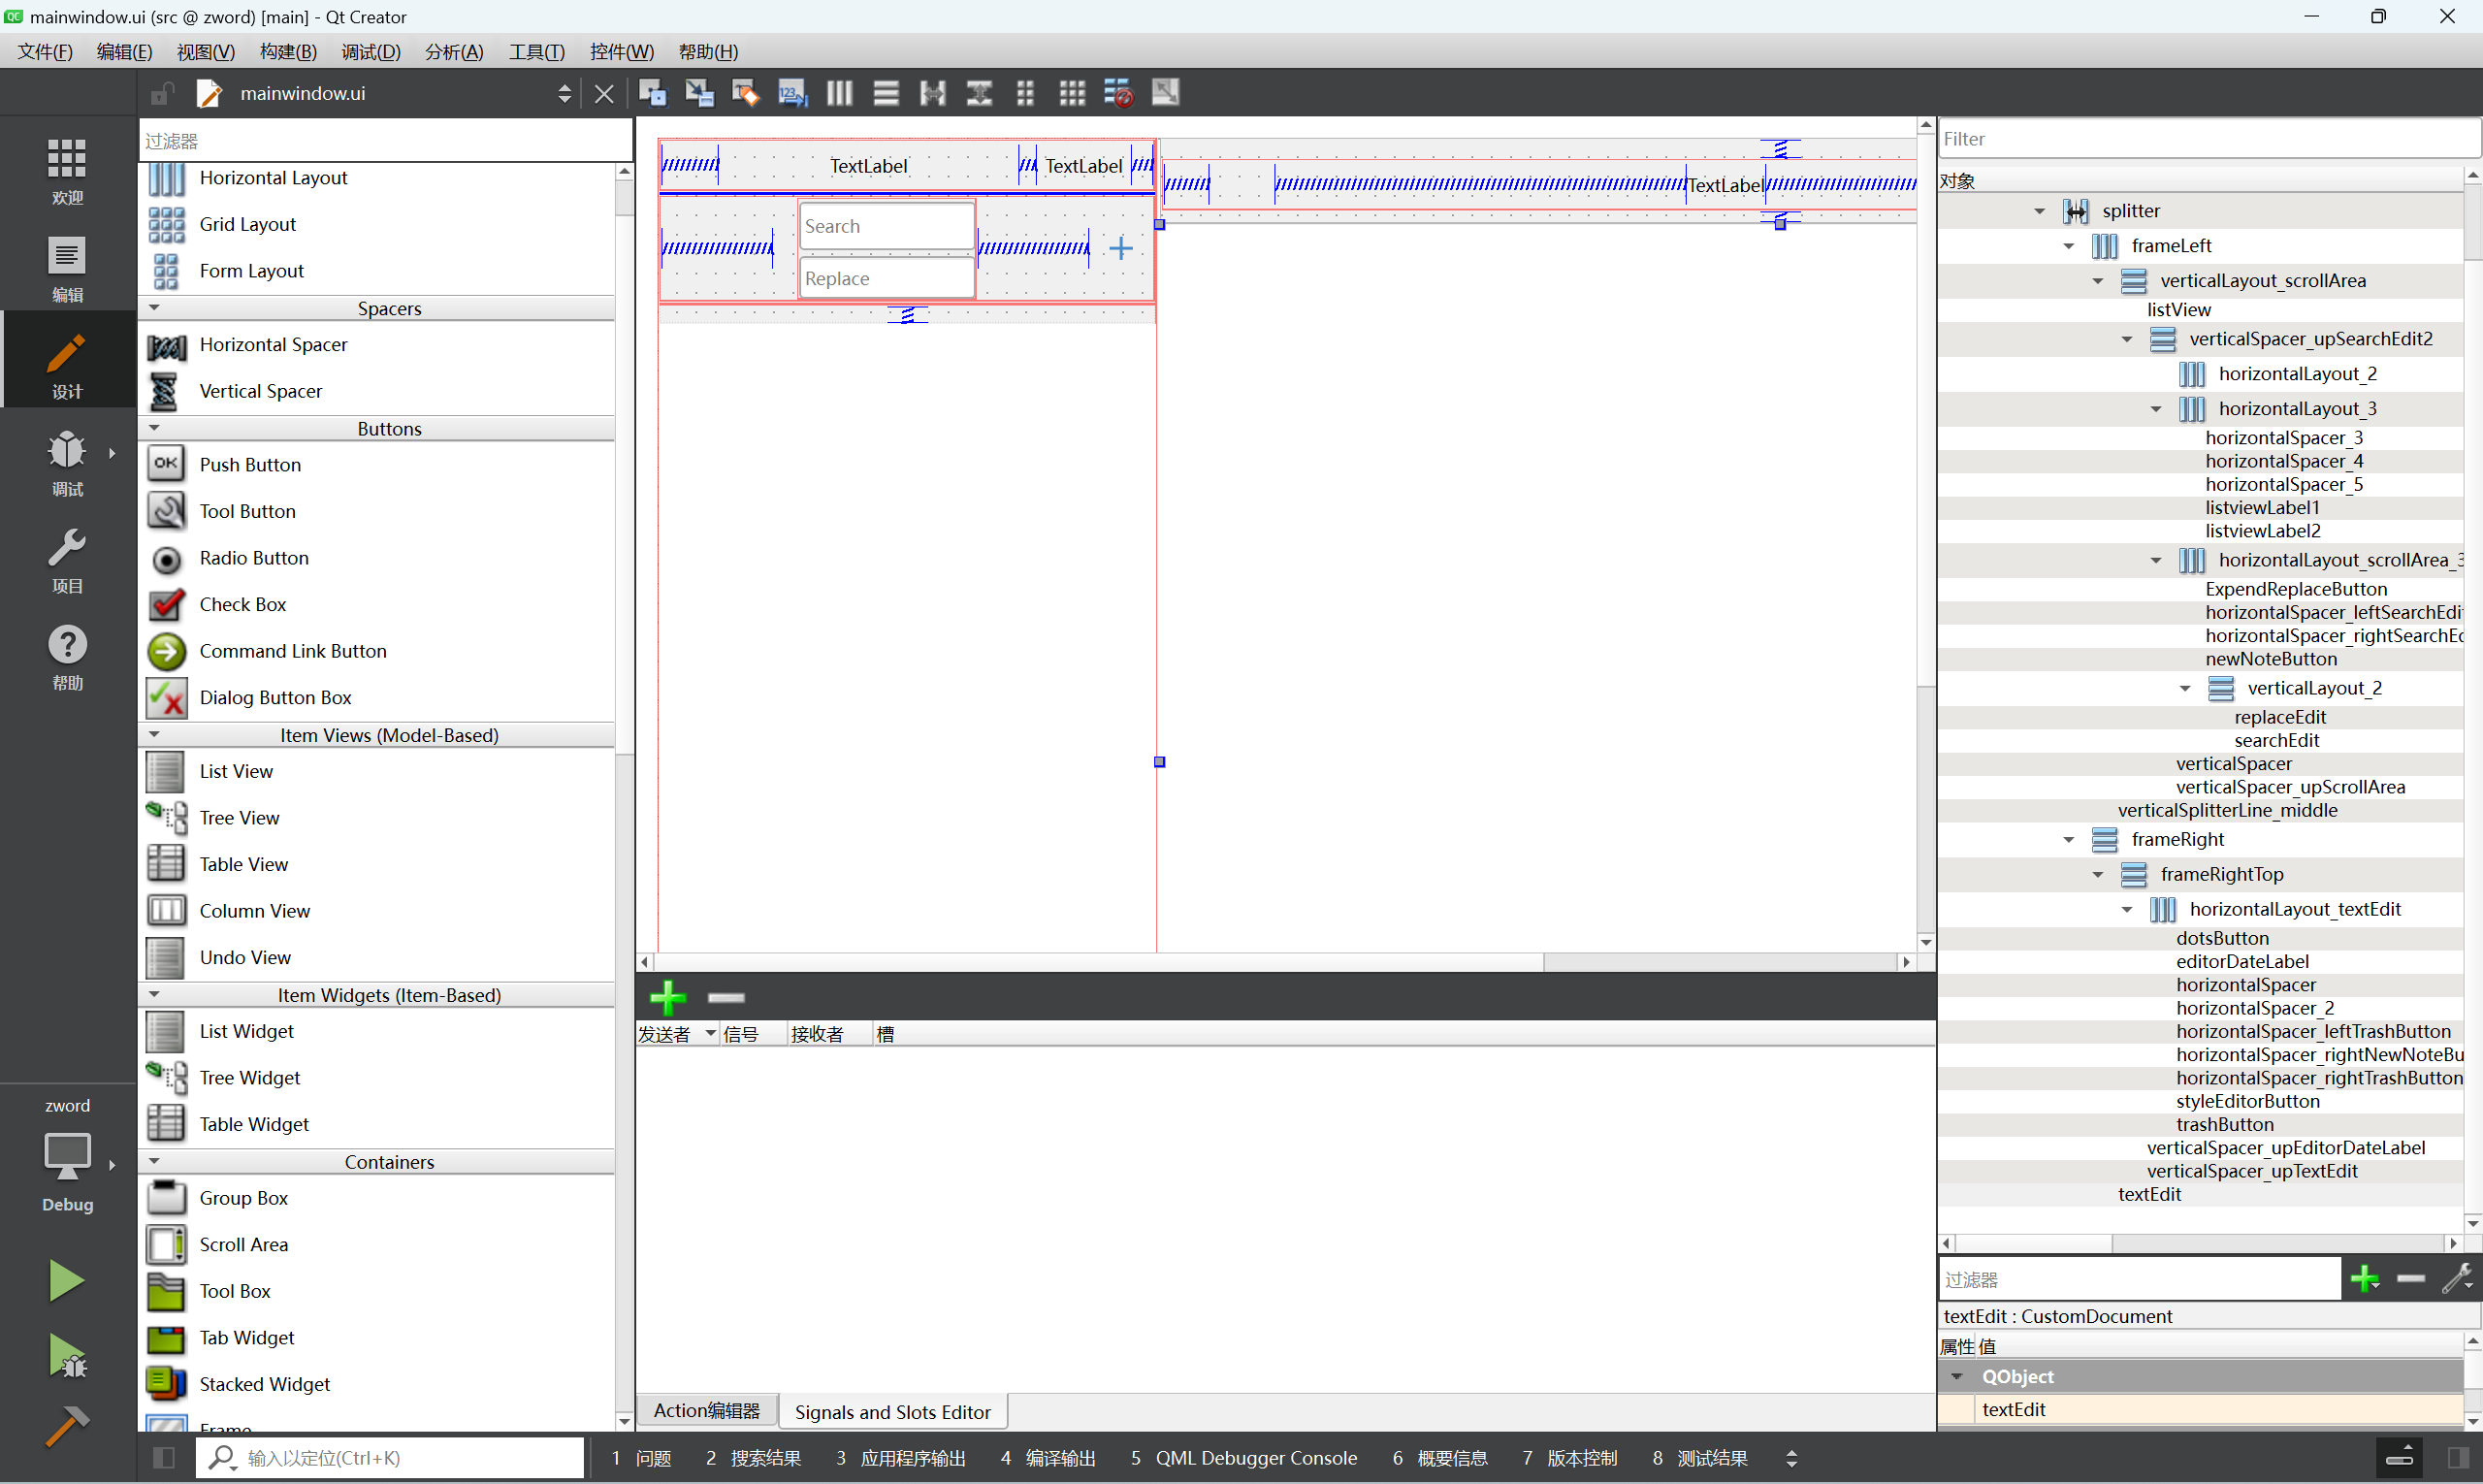
\includegraphics[width=2.5in]{1686925257848}
            \caption{界面设计:mainwindow.ui}
    \end{minipage}
\end{figure}
\subsubsection{保存文档的数据结构}
由于我们保存的格式为.txt纯文本格式,因此需要将格式保存为文本,类似markdown,因此最终考虑将文档保存为带格式原始文本和显示文本两种。其中带格式文本为全文本存储;显示文本为每一句一个字符串,并使用一个vector存储。\par
在每次打开文件和保存到本地文件的过程中,带格式文本进行更新,这个过程对长文本的处理相对较漫长。但当每次编辑时,显示文本能够实时更新,而且更新方式为:找到更改的文本段对应行字符串进行更改,如果添加和删除字符串再对后续文本段依次更新。这样处理文本的方式能够更加有效地处理长文本。\par
在源代码中定义了NodeData类,该类能够实现上述文本数据结构的构建。\par
文本的显示、输入等的用户交互界面我们主要使用Qt的QTextEdit进行。并以QTextEdit作为基类,派生出CustomDocument子类,进行如超链接等更多模块的拓展。\par
\subsubsection{文本格式设置}
由于主要的文本编辑显示窗口使用QTextEdit编辑,Qt中已经有很多非常基础的文本格式设置了,但这些格式的设置一来非常底层,二来只能够在显示的时候进行更改,不能保存到本地文件中,因此无法真正做到文本编辑器的功能。\par
考虑到我们保存为纯文本格式(txt),因此在保存文本格式的时候,可以借鉴Markdown一样的格式设置,通过特殊的符号和显示格式来实现简单格式的设置。\par
编译过程通过保存按键完成。\par
主要有以下三类文本格式:
\begin{itemize}
    \item 加粗和斜体格式。\par
    与Markdown的思路一样,通过在需要加粗和显示斜体文字前后加上相应符号。
    \item 文本总的字体、字号和颜色格式。\par
    我们设定为:同一个文本文件使用同一个字体、字号和颜色。字体、字号和颜色的格式放在每个文件的开头,以键值对字符串的方式存放,需要时通过读取字符串并进行对应格式转换实现。
    \item 段落对齐格式。\par
    在每个段落结束加上一个段落对齐的特殊符号以表示段落对齐格式。
\end{itemize}

\subsubsection{查找与替换}
使用了一个名为 SearchIterator 的类,用于在文本中查找指定的字符串。该类包含以下公共成员函数:

\begin{itemize}
    \item SearchIterator():默认构造函数,初始化成员变量。
    \item SearchIterator(QString\& search, QTextDocument* doc, int pos):构造函数,使用指定的搜索字符串、文本文档和起始位置初始化成员变量。
    \item void Init():初始化成员变量,将搜索位置和匹配位置都设置为 -1。
    \item $\sim$SearchIterator():析构函数,释放 next 数组的内存。
    \item SearchIterator\& operator=(const SearchIterator\& other):赋值运算符重载函数,用于将一个 SearchIterator 对象赋值给另一个对象。
    \item bool operator++():前缀自增运算符重载函数,用于查找下一个匹配字符串,返回值是为了区分末尾时匹配到字符的跳出与未匹配到字符的跳出,以此处理循环匹配。
    \item QTextCursor operator*():解引用运算符重载函数,返回当前匹配字符串的 QTextCursor 对象。
    \item bool operator==(const SearchIterator\& other):相等运算符重载函数,用于比较两个 SearchIterator 对象是否相等。
    \item bool operator!=(const SearchIterator\& other):不等运算符重载函数,用于比较两个 SearchIterator 对象是否不相等。
    \item bool operator==(const QString\& other):相等运算符重载函数,用于比较当前搜索字符串是否等于指定的字符串。
    \item bool operator!=(const QString\& other):不等运算符重载函数,用于比较当前搜索字符串是否不等于指定的字符串。
    \item int GetPos():返回当前匹配字符串的起始位置。
    \item bool IsEnd():判断是否已经搜索到文本末尾。
    \item bool IsHit():判断是否已经匹配到字符串,只要匹配到了字符串才会进行循环搜索。
    \item QString operator[](int pos):重载下标运算符,用于获取指定位置的字符。
\end{itemize}
此外,该类还包含了一些私有成员函数和变量,用于实现字符串匹配算法。其中,next 数组用于存储字符串匹配时的跳转表,text\_pos 和 pattern\_pos 分别表示当前搜索位置和匹配位置,text\_len 和 pattern\_len 分别表示文本长度和搜索字符串长度,cursor 表示当前搜索位置的 QTextCursor 对象,pattern 表示搜索字符串,hit\_at 表示匹配位置。

其内部使用了KMP字符串匹配算法,用于在一个文本串中查找一个模式串的出现位置。它的核心思想是利用已知信息来避免无效的比较,从而提高匹配效率。 KMP算法的实现基于一个跳转表(也称为失配函数或next数组),用于存储模式串中每个位置的最长公共前后缀长度,此表会在初始化时构建。KMP的时间复杂度为O(m+n),复杂度较低,尤其是在模式串较长时,效果更加明显。

% \begin{itemize}
%     \item 保存文档的数据结构
%     \item 如何处理连续输入文档时的内存分配情况,一次分配足够大还是每次都申请一段内存
%     \item 多级的撤销与重做,如何记录对文挡每次的操作
%     \item 如何表示文档中不同的文字格式
%     \item 如何记录段落格式
%     \item 支持多页文档的时候,如何进行分页
%     \item 汉字的储存和显示
% \end{itemize}

\section{系统模块说明}
%每一部分应有核心类说明
\subsection{界面}
界面总览如下:
\begin{figure}[!htbp]
    \begin{minipage}{0.45\textwidth}
        \centering
        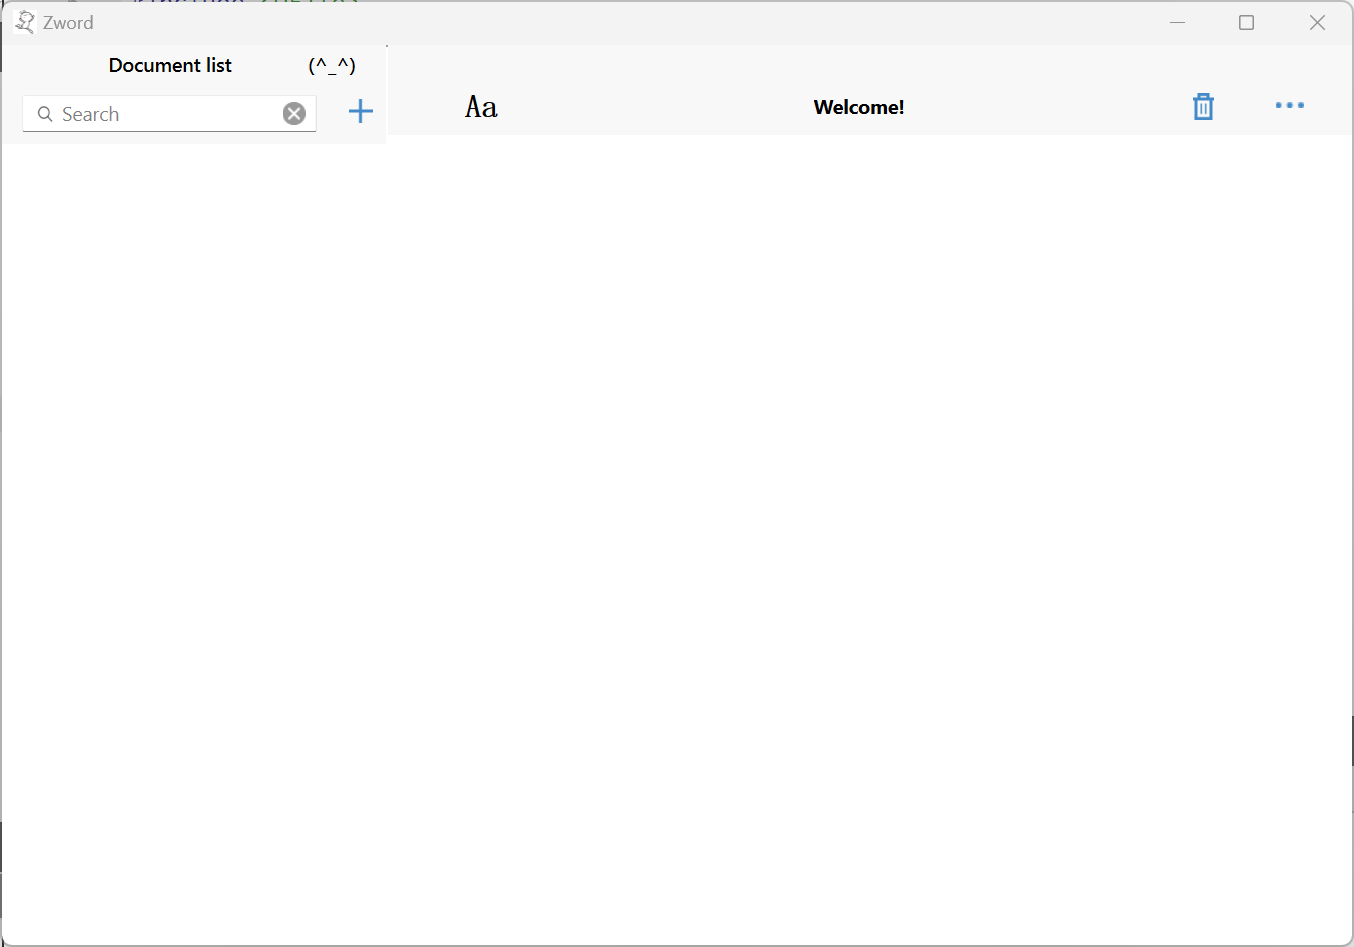
\includegraphics[width=2.5in]{1686455018197}
        \caption{空白界面}
    \end{minipage}
    \begin{minipage}{0.45\textwidth}
        \centering
        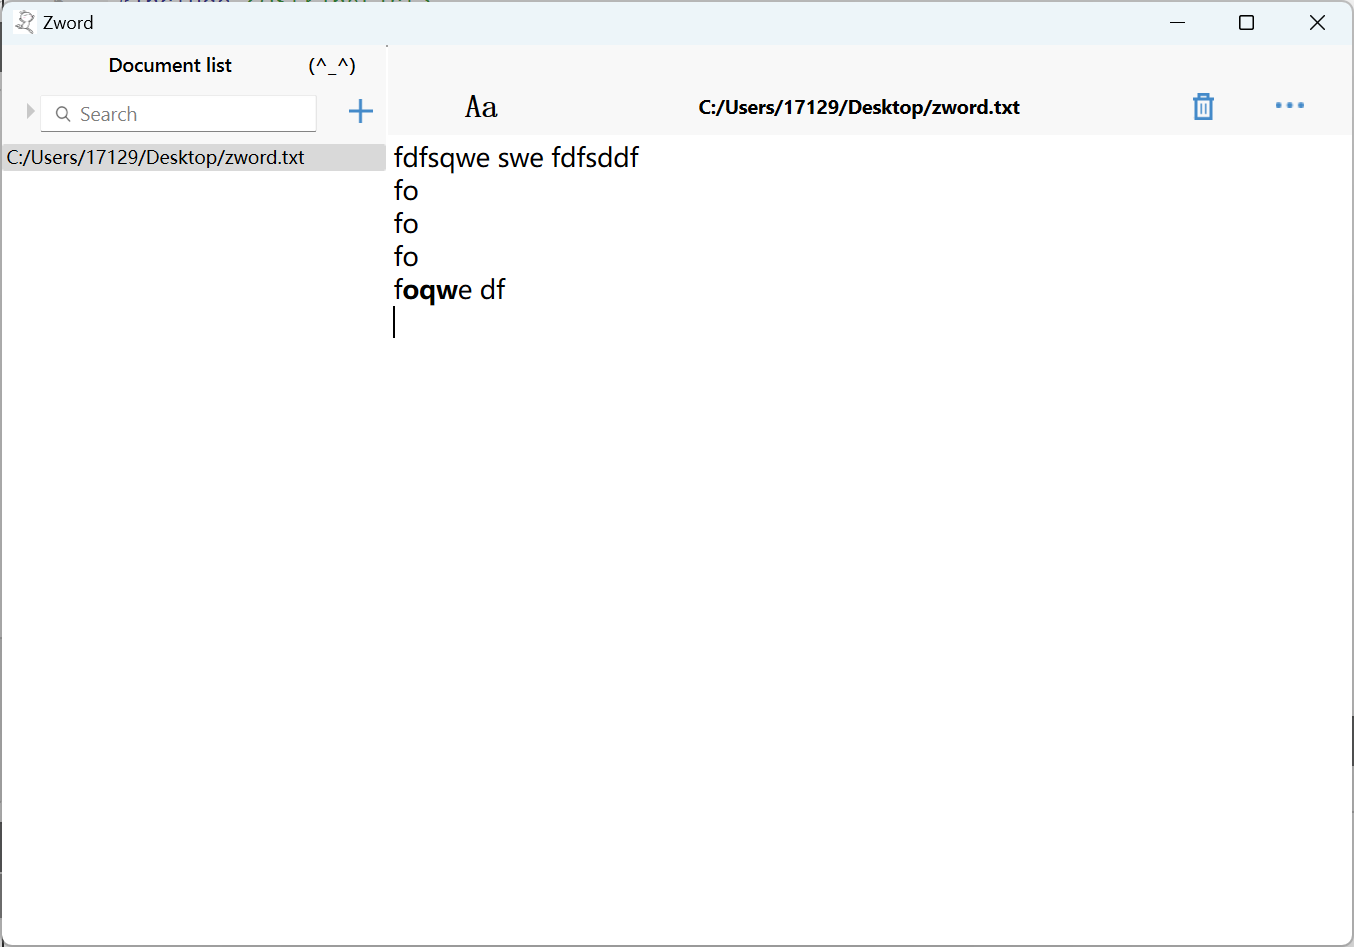
\includegraphics[width=2.5in]{1686842086143}
        \caption{加入文本界面}
    \end{minipage}
\end{figure}

主要的界面分为两个部分:左边是打开的文件列表,右边是文本输入区域\par
使用时,可以一次性打开多个文本文件,文件将会依次显示在左侧文件列表中,并通过鼠标单击的方式能够切换显示的不同文件。\par
右侧的文本输入区域能够进行文本编辑。十分推荐使用者在已有的文本或是新建文本上进行编辑操作。\par
上面的栏目为功能栏。其中,左上角的Search主要实现查找和替换功能模块,单击Search左侧的小箭头可以打开替换栏。功能栏上方有各种功能按键,其中右上角居中位置的字代表了当前工作中的文件名。
\subsection{文本基本操作}
\begin{itemize}
    \item 打开文本使用快捷键 Ctrl+O,只能打开已有文本
    \item 新建文本使用左上角的‘+’号,或者使用快捷键 Ctrl+N
    \item 保存文本使用快捷键 Ctrl+S
    \item 同其他文本编辑器一样,无法删除本地文本文件。若要删除当前打开的文本,可以点击右上角垃圾桶按钮或者使用快捷键 Ctrl+D
    \item 文本的撤销使用快捷键 Ctrl+Z,或者右键文本区选择 Undo
    \item 文本的重做使用快捷键 Ctrl+Y,或者右键文本区选择 Redo
    \item 文本的复制使用快捷键 Ctrl+C,或者右键文本区选择 Copy
    \item 文本的粘贴使用快捷键 Ctrl+V,或者右键文本区选择 Paste
    \item 文本的全选使用快捷键 Ctrl+A,或者右键文本区选择 Select All    
    \item 文本搜索使用快捷键 Ctrl+F,或左上角的搜索按钮
    \item 文本替换使用快捷键 Ctrl+H,或左上角展开后的替换按钮
    \item 文本的格式与颜色设置分别使用中间的两个按钮,为了实现的简单性,这两个按钮只能对整个文本进行设置,无法对文本的某一部分进行设置。
\end{itemize}

\subsection{文本格式操作}
\begin{itemize}
    \item 在文字的前后加上‘\#’号,再使用 Ctrl+S进行保存即可使‘\#’中间文本加粗。(带‘\#’的格式会保存到txt文本文件中,再次打开依然会显示该格式)
    \item 在文字的前后加上‘$\sim$’号,再使用 Ctrl+S进行保存即可使‘$\sim$’中间文本斜体。(带‘$\sim$’的格式会保存到txt文本文件中,再次打开依然会显示该格式)
    \item c++关键字能够高亮显示(格式不会保存到txt文本文件中)
    \item 对网址(正确url格式网址)按住 Ctrl键点击,能够使用默认浏览器访问该网址
    \item txt原始文本开始进行了字体等格式的设置
    \begin{figure}[!htbp]
        \centering
        \begin{minipage}{0.45\textwidth}
            \centering
            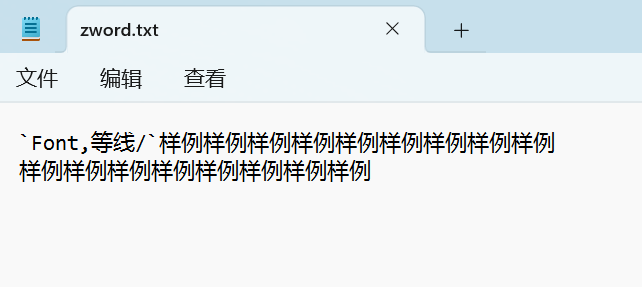
\includegraphics[width=2.5in]{1686456520111}
            \caption{开始进行字体格式设置}
        \end{minipage}
    \end{figure}
    \item 使用中间的 ‘Aa’按键可以选择文本字体和字体大小,选择的字体和大小会保存到txt文本文件中,再次打开也会显示该字体,但格式操作不会有效果。
    \item ‘Aa’旁边的按键可以设置文本的颜色。
    \item 文本设置为一行最多64个字符,如果调整窗口大小,可以看到文本能够自动缩进
    \item 使用最右上角的三个点按键,能够清除当前文本的所有格式,但只能在打开文本时点击。
    \item Ctrl+L Ctrl+E Ctrl+R三个快捷键能够进行段落的左、中、右对齐操作。其中,如果没有选中文本,将对所有文本段落进行对齐操作;如果选中文本,将对文本所在段进行对齐操作。保存后,段落对齐格式能够保存到txt文本文件中,再次打开也会显示该文本对齐格式。
\end{itemize}


\section{设计难点与解决方案}
\subsection{Qt学习与使用问题}
本次项目最大的难点还是在于Qt的学习和使用。由于Qt为使用者搭建了一个非常完整但同时很基本的开发环境,因此在实现文本编辑器的过程中,绝大时间都花费在通过官网和各类资源查找Qt某个具体函数的使用方法。而项目代码中的很大一部分都在调用Qt自带函数、重载或override其中某个基本函数等。

Qt的ui搭建使用的是Qt自带的ui设计器,因此在实现过程中,需要在ui设计器中添加各类控件,然后在代码中调用这些控件。这是首次搭建UI,使用的并不熟练,在过程中做了很多无用功。

\subsection{文本格式的保存}
另一个难点是文本格式的保存。因为需要处理带格式文本、不带格式纯文本和显示格式文本三类文本,因此在三类文本的相互转换和同步十分关键。而这里格式的显示和保存是一个双向的过程,既要实现打开一个txt文本文件能够显示格式,又要实现在文本编辑器中更改了文本格式后能够保存到txt文本文件中。

在具体的实现过程中,随着功能的增加和一开始结构设置的不完善,出现了很多代码的冗余,这也给后续功能的改进和实现产生了较大的负担。

此外,由于许多编辑器的功能是基于已保存的文本实现的,因此在实现过程中,需要注意在文本未保存时的各类操作的正确性。

\subsection{文本搜索的实现}
没有选择直接调用Qt自带的搜索函数,而是自己实现了一个搜索迭代器。这个迭代器主要使用了KMP算法。在实现过程中,由于KMP算法的特殊性,需要对文本进行预处理,因此需要注意迭代器的构造时next数字的构造与析构时的正确性。


\section{总结}

\newpage
\appendix

\section{项目开发日志}
\subsection{开发准备}
\subsubsection{环境配置}
使用 Qt6.5.0 配合 Qt Creator 或 VS2022 作为开发环境,\href{https://blog.csdn.net/m0_62919535/article/details/129340079}{配置 VS + Qt 的参考教程}。

\subsubsection{合作方式}
使用 github 开设私人仓库并设置合作者实现合作开发,可能使用 PR (Pull Requset) 实现更好的整合。

\subsubsection{文档写著}
使用 \LaTeX 进行文档的书写。

\subsection{项目搭建}


\end{document}